% ============================================================
%  速成讲义通用模板（已验证可编译：xelatex -no-pdf + xdvipdfmx）
%  用法：\documentclass 之后原样保留本节，正文用下面几个宏
% ============================================================
\documentclass[11pt,a4paper]{ctexart}
\usepackage[margin=2.1cm]{geometry}
\usepackage{amsmath,amssymb}
\usepackage{booktabs,array,tabularx}
\usepackage{xcolor}
\usepackage{enumitem}
\usepackage{tikz}
\usepackage{needspace}
\usepackage{multicol}
\setlength{\parindent}{0pt}
\setlist{itemsep=1pt,topsep=2pt,leftmargin=1.4em}

\definecolor{dark}{HTML}{222222}
% 黑底白字色块标题（章/大节）
\newcommand{\hd}[1]{\par\vspace{6pt}{\colorbox{dark}{\color{white}\bfseries\ #1\ }}\par\vspace{3pt}}
% 小标题
\newcommand{\sbm}[1]{\par\vspace{4pt}{\bfseries\color{dark}#1}\par\vspace{1pt}}
% 关键句（红）、定义（蓝）、行间公式（自动带间距）
\newcommand{\key}[1]{{\color{red}\bfseries #1}}
\newcommand{\dfn}[1]{{\color{blue}#1}}
\newcommand{\dm}[1]{\par\vspace{2pt}\[#1\]\vspace{2pt}\par}
% 单行要点：必须独占一段（LaTeX 单换行不换段）
\newcommand{\kk}[1]{\par\noindent\textbullet~#1\par}

\begin{document}
\begin{center}
{\LARGE\bfseries 速成讲义模板}\\[4pt]
{\small 宏测试页：色块标题 / 小标题 / 红字 / 蓝字 / 行间公式 / 要点，逐个走一遍}
\end{center}

\hd{第 1 章 示例章}
\sbm{1.1 定义与公式}
\dfn{定义}：这一段验证蓝色定义与中文混排、行间公式上下留白。

\dm{L_c=\frac{\lambda^2}{\Delta\lambda}=c\tau_c}
每一项：$L_c$ 相干长度；$\lambda$ 波长；$\Delta\lambda$ 谱宽；$\tau_c$ 相干时间。
\key{一句话}：谱线越窄，相干长度越长——傅里叶变换的必然。

\kk{要点一：一条要点写一次 kk，命令不能嵌套，也不能用单换行并列。}
\kk{要点二：中文里的希腊字母一律进数学模式，否则 \small 里不渲染。}

\begin{center}
\begin{tabular}{@{}llr@{}}
\toprule
量 & 符号 & 数值 \\
\midrule
相干长度 & $L_c$ & 0.36\,mm \\
波数 & $\tilde\nu=s/2L$ & --- \\
\bottomrule
\end{tabular}
\end{center}
% 表格前若有引导句，句末加 \par 或空行，否则被当成行内盒子冲出页边

\begin{center}
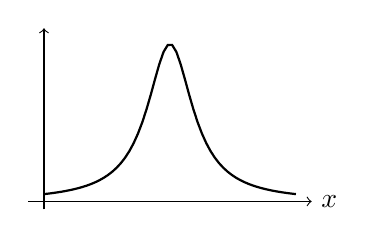
\begin{tikzpicture}[x=1cm,y=2cm]
\draw[->] (-0.2,0)--(3.4,0) node[right]{$x$};
\draw[->] (0,-0.05)--(0,1.1);
\draw[thick] plot[domain=0:3.2,samples=60] (\x,{1/(1+8*(\x-1.6)^2)});
\end{tikzpicture}
\end{center}

\end{document}